\documentclass[doku]{subfiles}
\begin{document}
	\subsection{常用综合超市}
	在科布伦茨常见的综合类超市有REWE,Penny, Edeka, Lidi, ALDI,Netto。\\
	Edeka我觉得价格是最高的一家,感觉提供的蔬菜种类和质量还是比较高的,超市装修的也比较好, Rewe价格稍次于Edeka,他们提供的蔬菜和水果种类稍逊于Edeka,但总体质量和数量都还是不错的,这两家除了统一的肉柜,还有人工售卖的肉柜,
	
	\begin{figure}
		\centering
		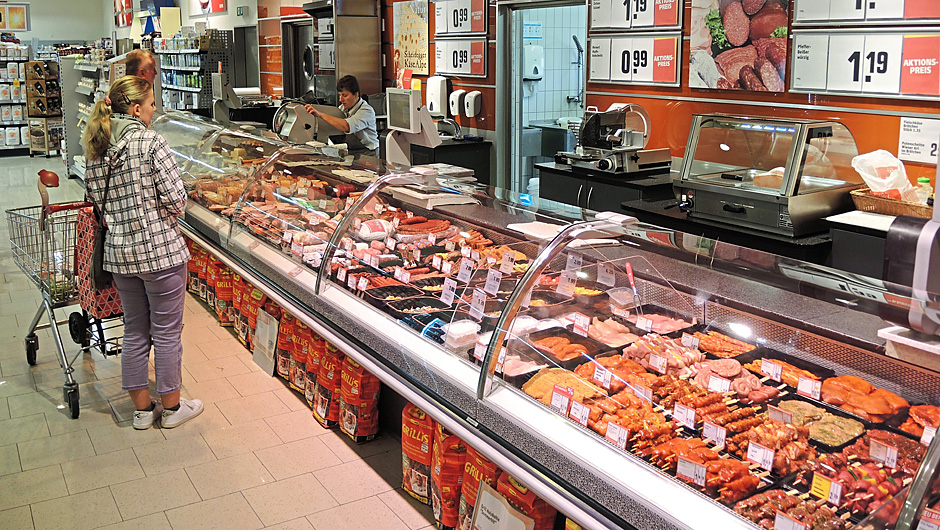
\includegraphics[width=0.7\linewidth]{Fleischtheke-bei-Rewe-154924}
		\caption{人工肉柜}
		\label{fig:fleischtheke-bei-rewe-154924}
	\end{figure}
	\begin{figure}
		\centering
		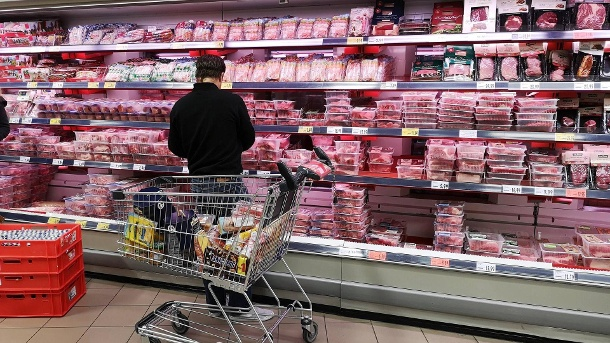
\includegraphics[width=0.7\linewidth]{Regal-Fleisch}
		\caption{冰箱肉柜}
		\label{fig:regal-fleisch}
	\end{figure}
	
	在那里可以和店员订一些不常见的东西,例如猪的juejue。 Lidi我接触的不多,定位也不大了解,只是去过两次买肋排,剩下的Penny,ALDI,Netto是标准的所谓的“廉价”超市,相比于最开始的两者,这几个超市只有标准冰箱的那种肉柜,提供的都是一些标准化包装和固定种类的商品,因此价格会稍微低一些,但是这样的超市有一个特点是每周都会提供一些只有这周才有的商品,而且价格是很实惠的,例如Penny时不时有的猪肘啦(大晚上饿了),一个猪肘不到3欧,红烧一下还是很带劲的,但是这样的东西需要自己多注意,我经常路过的时候会去超市顺一个宣传册,当然在网上也可以搜到的\href{https://www.prospektangebote.de/}{prospektangebote},在这些综合类超市里,你除了可以买到基本的吃喝类的商品,基本的日化用品也是可以买得到的,例如洗发,沐浴里,面膜,电池,胶水,blabla,但种类都十分有限。
	
	\subsubsection{Amazon}
	\begin{figure}[h]
		\centering
		
\includegraphics[width=0.56\linewidth]{amazon}
		\caption{Amazon}
		\label{fig:amazon}
	\end{figure}
	亚马逊就当JD来看吧,东西还是比较全的,而且运送时效都还不错,但是亚马逊的价格基本上都是偏高的。
	
	\subsection{日化用品}
	\subsubsection{dm}
	\begin{figure}[h]
		\centering
		
\includegraphics[width=0.4\linewidth]{dm}
		\caption{dm}
		\label{fig:dm}
	\end{figure}
	
	拍在最头上的必然就是dm,你生活中所用到的大部分日用品都能在dm买到,像是厨房里的洗洁精,海绵,洗衣服用的香氛,洗衣液,女生的染发的,面膜,护手霜什么的,以及婴儿用品,除了这些日化用品还有一些健康保健用品(棉棒),顺便说一下泡腾片,在德国果蔬摄入肯定没有国内多,还是有必要通过泡腾片再补充一些,还有一些Bio的食物,更多是小饼干和麦片的那类东西,当然还有目前最重要的口罩和消毒液,除此之外,dm还可以打印照片,但是不得不说在现场印的那种质量不是很好,我比较推荐,在网上的dm里下单,然后选择到店取,或者邮寄,到店自取的优点是不需要邮费。 如果有喜欢拍点胶卷的,dm也是可以洗胶卷的~~~~ 这个也是我在这里呆了好久之后,朋友告诉我才知道的,你只需要填一个信封,这个信封在dm的照片区域能找到,把你的胶卷放到信封里,然后就可以扔到一个小洞里,过个一两周就可以去dm的柜子里找。我冲的胶卷基本都是一周就可以取了。然鹅。。目前全德dm的胶卷都断货中,德国的KodakGold200有的时候还是很便宜的,虽然比国内便宜,但是请不要借此,进行倒卖!!!请不要破坏市场。
	\begin{figure}
		\centering
		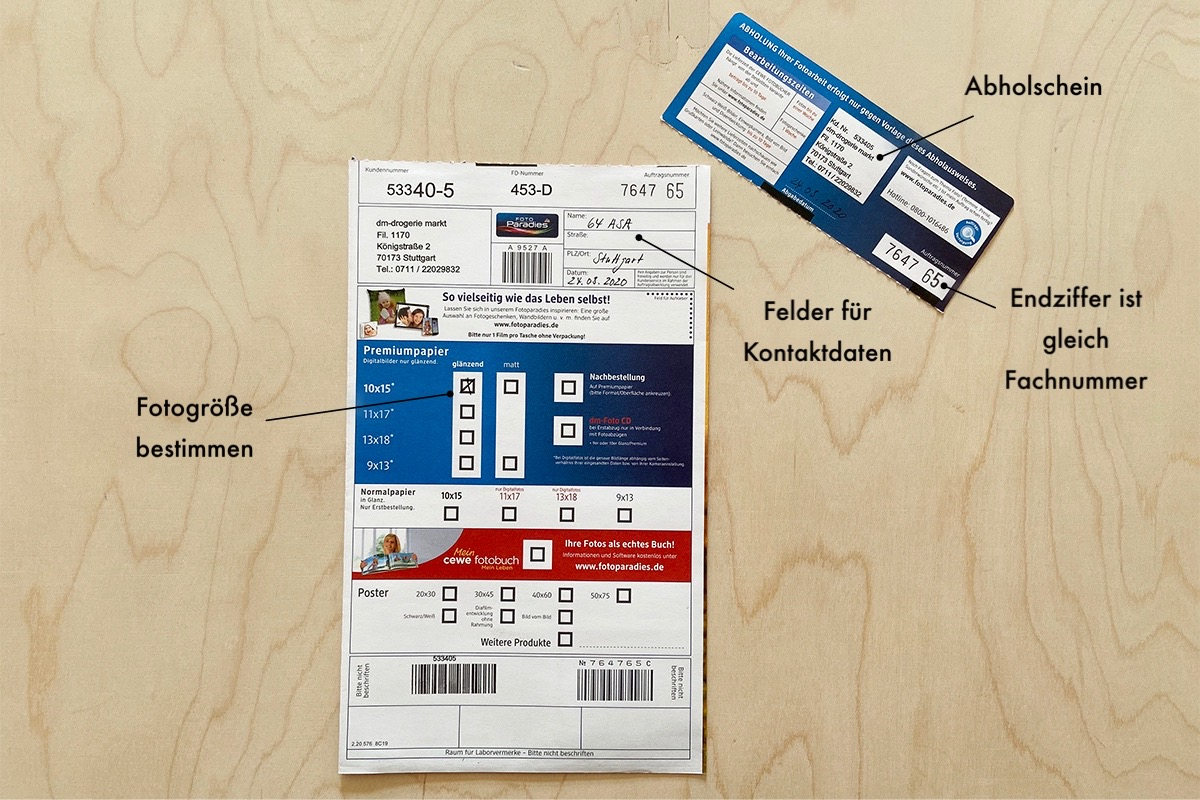
\includegraphics[width=0.35\linewidth]{analogfilm}
		\caption{胶卷信封}
		\label{fig:analogfilm}
	\end{figure}

	总结一下dm,在日化方面,你所需的$98\%$都可以在dm找到。
	
	\subsubsection{Müller}
	\begin{figure}[h]
		\centering
		
\includegraphics[width=0.7\linewidth]{mueller}
		\caption{Müller}
		\label{fig:mueller}
	\end{figure}
	
	Müller 里的日用品只是其中一个小分类了,Müller的一楼(EG),有各式各样的化妆品,请自行,探索,问我白问。。。二楼是玩具一类的,三楼是办公用品也就是我们说的本子啦,笔啦,这样的学习用品都可以在这里买,我一般去Müller都是二话不说直奔三楼。。负一楼是类似于dm的日用品销售。 
	\subsection{电子商店}
	\subsubsection{Satrun und MediaMarkt}
	\begin{figure}
		\centering
		
\includegraphics[width=0.6\linewidth]{saturnMedia}
		\caption{Saturn und MediaMarkt}
		\label{fig:saturnmedia}
	\end{figure}
	
	这两家都是经营各类电子产品产品,厨房电器,电视显示器,电脑手机,各类配件都是可以在这里买的到的,据说这两还是一家。。。我。。。
	
	\subsubsection{Cyberport}
	Cyberport\href{https://www.cyberport.de/}{Url},听这个名字就很赛博朋克,这个店只有网店,虽然我没有用过,但是应该即将会用他来买打印机,因为Payback\footnote{Payback是德国十分流行的积分卡,你可以在很多超市里获得积分,不要不好意思,当时上语言课还讨论过这个,对比东方和西方的意识形态,这个都是各个公司给付过钱的东西,超市很乐意顾客使用,柜员都会问你你有payback嘛}的积分可以换这里的消费券。这里也是可以购买很多电子产品,但是感觉这里更侧重手机,电脑,打印机这类消费品。
	
	\subsubsection{Conrad}
	\begin{figure}[h]
		\centering
		
\includegraphics[width=0.58\linewidth]{Conrad-Electronic-Logo.svg}
		\caption{Conrad}
		\label{fig:conrad-electronic-logo}
	\end{figure}
	
	作为自动化的学生,想买原件在哪买,当然可以ebay,但是ebay的分类在搜索元器件时不是那么的省心,这时不得不提一下Conrad\href{https://www.conrad.de/}{URL},Conrad更多是面向DIY人群,这里你不光能能买到小的元器件,还能买到树莓派,三维相机,3D打印机等这一类偏向于极客类的产品,在这里搜索元器件,分类十分清晰,哈哈,但是这里价格稍微偏高,我一般都是在这里找到型号,然后复制名字,去ebay里再搜和购买~\label{conrad}
	
	\subsection{吃喝玩乐}
	\subsubsection{Forum}
	\begin{figure}
		\centering
		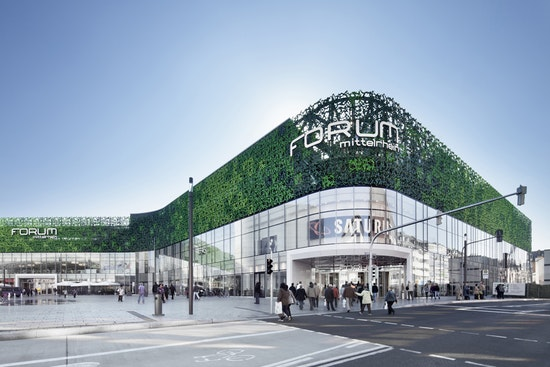
\includegraphics[width=0.6\linewidth]{forum}
		\caption{Forum}
		\label{fig:forum}
	\end{figure}
	
	Forum \ref{fig:forum}是科布伦茨的的。。。的。。。万象城,哈楼上有吃的,中间有迪卡侬和HM,负一楼有TEDI\footnote{Tedi 是一个卖居家用品的廉价超市。。。德国的一元店,虽然质量我真的只能是呵呵了},Saturn,DM。
	
	\subsection{Lockdown}
	目前预计Lockdown持续到三月七日,所以你们来的时候有些特殊要求你们还是应该稍微了解一下。目前除了超市(REWE,Penny这一类)和日化用品店(DM)外的所有的商店都是关闭的,其他的店都只有网购,进入超市需要注意,必须要戴口罩,理论上还是要推车的,因为推车可以保证人与人之间的间隔,虽然推车这个现在没有20年初那么严格,但是还是尽量遵守吧。\label{lockdown-markt}
	
\end{document}